% Options for packages loaded elsewhere
\PassOptionsToPackage{unicode}{hyperref}
\PassOptionsToPackage{hyphens}{url}
%
\documentclass[
]{article}
\usepackage{lmodern}
\usepackage{amssymb,amsmath}
\usepackage{ifxetex,ifluatex}
\ifnum 0\ifxetex 1\fi\ifluatex 1\fi=0 % if pdftex
  \usepackage[T1]{fontenc}
  \usepackage[utf8]{inputenc}
  \usepackage{textcomp} % provide euro and other symbols
\else % if luatex or xetex
  \usepackage{unicode-math}
  \defaultfontfeatures{Scale=MatchLowercase}
  \defaultfontfeatures[\rmfamily]{Ligatures=TeX,Scale=1}
\fi
% Use upquote if available, for straight quotes in verbatim environments
\IfFileExists{upquote.sty}{\usepackage{upquote}}{}
\IfFileExists{microtype.sty}{% use microtype if available
  \usepackage[]{microtype}
  \UseMicrotypeSet[protrusion]{basicmath} % disable protrusion for tt fonts
}{}
\makeatletter
\@ifundefined{KOMAClassName}{% if non-KOMA class
  \IfFileExists{parskip.sty}{%
    \usepackage{parskip}
  }{% else
    \setlength{\parindent}{0pt}
    \setlength{\parskip}{6pt plus 2pt minus 1pt}}
}{% if KOMA class
  \KOMAoptions{parskip=half}}
\makeatother
\usepackage{xcolor}
\IfFileExists{xurl.sty}{\usepackage{xurl}}{} % add URL line breaks if available
\IfFileExists{bookmark.sty}{\usepackage{bookmark}}{\usepackage{hyperref}}
\hypersetup{
  pdftitle={Practicality of Statistical Inference},
  pdfauthor={Anandu R},
  hidelinks,
  pdfcreator={LaTeX via pandoc}}
\urlstyle{same} % disable monospaced font for URLs
\usepackage[margin=1in]{geometry}
\usepackage{color}
\usepackage{fancyvrb}
\newcommand{\VerbBar}{|}
\newcommand{\VERB}{\Verb[commandchars=\\\{\}]}
\DefineVerbatimEnvironment{Highlighting}{Verbatim}{commandchars=\\\{\}}
% Add ',fontsize=\small' for more characters per line
\usepackage{framed}
\definecolor{shadecolor}{RGB}{248,248,248}
\newenvironment{Shaded}{\begin{snugshade}}{\end{snugshade}}
\newcommand{\AlertTok}[1]{\textcolor[rgb]{0.94,0.16,0.16}{#1}}
\newcommand{\AnnotationTok}[1]{\textcolor[rgb]{0.56,0.35,0.01}{\textbf{\textit{#1}}}}
\newcommand{\AttributeTok}[1]{\textcolor[rgb]{0.77,0.63,0.00}{#1}}
\newcommand{\BaseNTok}[1]{\textcolor[rgb]{0.00,0.00,0.81}{#1}}
\newcommand{\BuiltInTok}[1]{#1}
\newcommand{\CharTok}[1]{\textcolor[rgb]{0.31,0.60,0.02}{#1}}
\newcommand{\CommentTok}[1]{\textcolor[rgb]{0.56,0.35,0.01}{\textit{#1}}}
\newcommand{\CommentVarTok}[1]{\textcolor[rgb]{0.56,0.35,0.01}{\textbf{\textit{#1}}}}
\newcommand{\ConstantTok}[1]{\textcolor[rgb]{0.00,0.00,0.00}{#1}}
\newcommand{\ControlFlowTok}[1]{\textcolor[rgb]{0.13,0.29,0.53}{\textbf{#1}}}
\newcommand{\DataTypeTok}[1]{\textcolor[rgb]{0.13,0.29,0.53}{#1}}
\newcommand{\DecValTok}[1]{\textcolor[rgb]{0.00,0.00,0.81}{#1}}
\newcommand{\DocumentationTok}[1]{\textcolor[rgb]{0.56,0.35,0.01}{\textbf{\textit{#1}}}}
\newcommand{\ErrorTok}[1]{\textcolor[rgb]{0.64,0.00,0.00}{\textbf{#1}}}
\newcommand{\ExtensionTok}[1]{#1}
\newcommand{\FloatTok}[1]{\textcolor[rgb]{0.00,0.00,0.81}{#1}}
\newcommand{\FunctionTok}[1]{\textcolor[rgb]{0.00,0.00,0.00}{#1}}
\newcommand{\ImportTok}[1]{#1}
\newcommand{\InformationTok}[1]{\textcolor[rgb]{0.56,0.35,0.01}{\textbf{\textit{#1}}}}
\newcommand{\KeywordTok}[1]{\textcolor[rgb]{0.13,0.29,0.53}{\textbf{#1}}}
\newcommand{\NormalTok}[1]{#1}
\newcommand{\OperatorTok}[1]{\textcolor[rgb]{0.81,0.36,0.00}{\textbf{#1}}}
\newcommand{\OtherTok}[1]{\textcolor[rgb]{0.56,0.35,0.01}{#1}}
\newcommand{\PreprocessorTok}[1]{\textcolor[rgb]{0.56,0.35,0.01}{\textit{#1}}}
\newcommand{\RegionMarkerTok}[1]{#1}
\newcommand{\SpecialCharTok}[1]{\textcolor[rgb]{0.00,0.00,0.00}{#1}}
\newcommand{\SpecialStringTok}[1]{\textcolor[rgb]{0.31,0.60,0.02}{#1}}
\newcommand{\StringTok}[1]{\textcolor[rgb]{0.31,0.60,0.02}{#1}}
\newcommand{\VariableTok}[1]{\textcolor[rgb]{0.00,0.00,0.00}{#1}}
\newcommand{\VerbatimStringTok}[1]{\textcolor[rgb]{0.31,0.60,0.02}{#1}}
\newcommand{\WarningTok}[1]{\textcolor[rgb]{0.56,0.35,0.01}{\textbf{\textit{#1}}}}
\usepackage{graphicx,grffile}
\makeatletter
\def\maxwidth{\ifdim\Gin@nat@width>\linewidth\linewidth\else\Gin@nat@width\fi}
\def\maxheight{\ifdim\Gin@nat@height>\textheight\textheight\else\Gin@nat@height\fi}
\makeatother
% Scale images if necessary, so that they will not overflow the page
% margins by default, and it is still possible to overwrite the defaults
% using explicit options in \includegraphics[width, height, ...]{}
\setkeys{Gin}{width=\maxwidth,height=\maxheight,keepaspectratio}
% Set default figure placement to htbp
\makeatletter
\def\fps@figure{htbp}
\makeatother
\setlength{\emergencystretch}{3em} % prevent overfull lines
\providecommand{\tightlist}{%
  \setlength{\itemsep}{0pt}\setlength{\parskip}{0pt}}
\setcounter{secnumdepth}{-\maxdimen} % remove section numbering

\title{Practicality of Statistical Inference}
\author{Anandu R}
\date{8/25/2020}

\begin{document}
\maketitle

\hypertarget{examples-of-pdfs}{%
\subsection{examples of PDFs}\label{examples-of-pdfs}}

\hypertarget{example-1}{%
\subsubsection{Example 1}\label{example-1}}

Consider the function to denote the probability of help calls addressed
by a helpline be

\begin{verbatim}
  f(x) = {2x for 0<x<1; 0 otherwise}
\end{verbatim}

\includegraphics{statisticalInference_files/figure-latex/unnamed-chunk-1-1.pdf}

To find probability that 75\% or fewer of calls get addressed

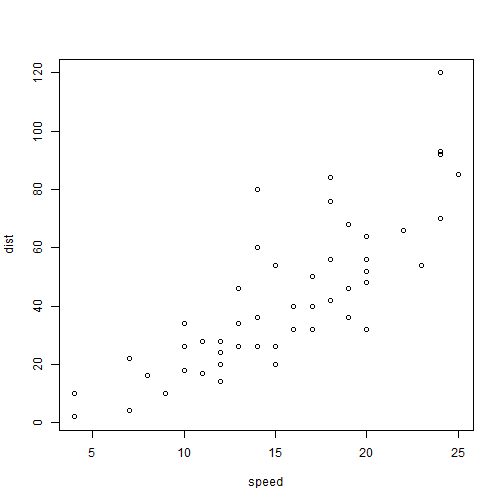
\includegraphics{statisticalInference_files/figure-latex/unnamed-chunk-2-1.pdf}

Find area of given portion

\begin{verbatim}
  (1/2)*(0.75)*(1.5)
  = 0.5625
\end{verbatim}

The same can be achieved by using the beta function for probability -
pbeta()

\begin{Shaded}
\begin{Highlighting}[]
\KeywordTok{pbeta}\NormalTok{(}\FloatTok{0.75}\NormalTok{,}\DecValTok{2}\NormalTok{,}\DecValTok{1}\NormalTok{)}
\end{Highlighting}
\end{Shaded}

The quantile for the above population distribution\\
Median from the distribution shows the datapoint below which 50\% of the
data is present and above it is the other 50\%

\begin{verbatim}
  0.5 = F(X) = P(X<=x) = 50% of the area
  Integrating the function F(X)=2x, we get x^2
  => x = sqrt(2) = 0.707
  => The required datapoint
\end{verbatim}

The same can be found out using the qbeta() function which gives the
quantile of the beta distribution

\begin{Shaded}
\begin{Highlighting}[]
\KeywordTok{qbeta}\NormalTok{(}\FloatTok{0.5}\NormalTok{,}\DecValTok{2}\NormalTok{,}\DecValTok{1}\NormalTok{)}
\end{Highlighting}
\end{Shaded}

The inference is that during 50\% of the day \textasciitilde70\% of the
calls are addressed.

\hypertarget{real-world-example-of-statistical-inference}{%
\subsection{Real World Example of Statistical
Inference}\label{real-world-example-of-statistical-inference}}

Using the Son's Height attribute from the father.son data

\hypertarget{loading-the-data}{%
\subsubsection{Loading the data}\label{loading-the-data}}

\begin{Shaded}
\begin{Highlighting}[]
\CommentTok{## Loading the data}
\KeywordTok{suppressMessages}\NormalTok{(}
\NormalTok{  \{}
    \ControlFlowTok{if}\NormalTok{(}\OperatorTok{!}\KeywordTok{require}\NormalTok{(}\StringTok{'UsingR'}\NormalTok{))\{}
      \KeywordTok{install.packages}\NormalTok{(}\StringTok{'UsingR'}\NormalTok{)}
      \KeywordTok{library}\NormalTok{(UsingR); }\KeywordTok{data}\NormalTok{(father.son)}
\NormalTok{    \}}
    \ControlFlowTok{if}\NormalTok{(}\OperatorTok{!}\KeywordTok{require}\NormalTok{(}\StringTok{'dplyr'}\NormalTok{))\{}
      \KeywordTok{install.packages}\NormalTok{(}\StringTok{"dplyr"}\NormalTok{)}
      \KeywordTok{library}\NormalTok{(dplyr)}
\NormalTok{    \}}
\NormalTok{  \}}
\NormalTok{)}
\NormalTok{x =}\StringTok{ }\NormalTok{father.son}\OperatorTok{$}\NormalTok{sheight}
\NormalTok{n =}\StringTok{ }\KeywordTok{length}\NormalTok{(x)}
\end{Highlighting}
\end{Shaded}

\hypertarget{plot-of-heights}{%
\subsubsection{Plot of heights}\label{plot-of-heights}}

\begin{Shaded}
\begin{Highlighting}[]
\KeywordTok{ggplot}\NormalTok{() }\OperatorTok{+}\StringTok{ }\KeywordTok{geom_histogram}\NormalTok{(}\KeywordTok{aes}\NormalTok{(x), }\DataTypeTok{col =} \StringTok{"white"}\NormalTok{, }\DataTypeTok{fill =} \StringTok{"skyblue"}\NormalTok{) }\OperatorTok{+}\StringTok{ }\KeywordTok{theme_bw}\NormalTok{()}
\end{Highlighting}
\end{Shaded}

\begin{verbatim}
## `stat_bin()` using `bins = 30`. Pick better value with `binwidth`.
\end{verbatim}

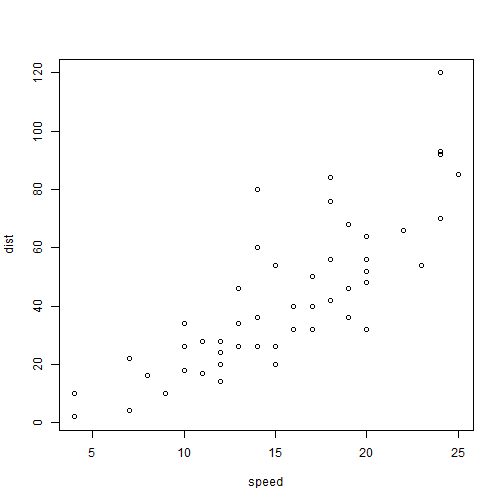
\includegraphics{statisticalInference_files/figure-latex/unnamed-chunk-6-1.pdf}

The height is represented in feet instead of inches, divide the height
by 12 to convert to feet unit

\begin{Shaded}
\begin{Highlighting}[]
\KeywordTok{round}\NormalTok{(}\KeywordTok{c}\NormalTok{(}\KeywordTok{var}\NormalTok{(x),}\KeywordTok{var}\NormalTok{(x)}\OperatorTok{/}\NormalTok{n,}\KeywordTok{sd}\NormalTok{(x),}\KeywordTok{sd}\NormalTok{(x)}\OperatorTok{/}\KeywordTok{sqrt}\NormalTok{(n)),}\DecValTok{2}\NormalTok{)}
\end{Highlighting}
\end{Shaded}

\begin{verbatim}
## [1] 7.92 0.01 2.81 0.09
\end{verbatim}

\hypertarget{explaining-confidence-intervals}{%
\subsection{Explaining confidence
intervals}\label{explaining-confidence-intervals}}

\begin{Shaded}
\begin{Highlighting}[]
\NormalTok{(}\KeywordTok{mean}\NormalTok{(x)}\OperatorTok{+}\KeywordTok{c}\NormalTok{(}\OperatorTok{-}\DecValTok{1}\NormalTok{,}\DecValTok{1}\NormalTok{)}\OperatorTok{*}\KeywordTok{qnorm}\NormalTok{(}\FloatTok{0.975}\NormalTok{)}\OperatorTok{*}\KeywordTok{sd}\NormalTok{(x)}\OperatorTok{/}\KeywordTok{sqrt}\NormalTok{(}\KeywordTok{length}\NormalTok{(x)))}\OperatorTok{/}\DecValTok{12}
\end{Highlighting}
\end{Shaded}

\begin{verbatim}
## [1] 5.709670 5.737674
\end{verbatim}

This tells us that if we were to iid draw the sons from this population
the CI for drawing an average height to the sons would in the interval
5.71 to 5.74

\textbf{Sample Proportions}: In an event that each Xi is 0 or 1(binary
outcome), with common success probability p, then variance(sigma\^{}2) =
p(1-p)\\
Then the interval takes the form\\
Wald confidence interval for p - For 95\% intervals is:

\begin{verbatim}
  ^p (+/-) 1/sqrt(n)
\end{verbatim}

which is a quick CI estimate for p

\hypertarget{confidence-interval-example}{%
\subsection{Confidence interval
example}\label{confidence-interval-example}}

Your campaign advisor told you that in a random sample of 100 likely
voters, 56 intend to vote for you. - Can you relax? Do you have this
race in the bag? - without access to a computer or calculator, how
precise is the estimate?

Using Wald confidence, 1/(sqrt(100)) gives 0.1 confidence interval of
{[}0.46,0.66{]} - Not enoug for you to relax, we can't rule out
possibilities below 0.5 with 95\% confidence, better go do more
campaigning.

The above calculation of CI can be done using the binom.test() function
in R

\begin{Shaded}
\begin{Highlighting}[]
\KeywordTok{binom.test}\NormalTok{(}\DecValTok{56}\NormalTok{,}\DecValTok{100}\NormalTok{)}\OperatorTok{$}\NormalTok{conf.int}
\end{Highlighting}
\end{Shaded}

\begin{verbatim}
## [1] 0.4571875 0.6591640
## attr(,"conf.level")
## [1] 0.95
\end{verbatim}

Yielding a similar result as before. Mathematically which is

\begin{Shaded}
\begin{Highlighting}[]
\FloatTok{0.56} \OperatorTok{+}\StringTok{ }\KeywordTok{c}\NormalTok{(}\OperatorTok{-}\DecValTok{1}\NormalTok{,}\DecValTok{1}\NormalTok{)}\OperatorTok{*}\KeywordTok{qnorm}\NormalTok{(}\FloatTok{0.975}\NormalTok{)}\OperatorTok{*}\KeywordTok{sqrt}\NormalTok{(}\FloatTok{0.56}\OperatorTok{*}\FloatTok{0.44}\OperatorTok{/}\DecValTok{100}\NormalTok{)}
\end{Highlighting}
\end{Shaded}

\begin{verbatim}
## [1] 0.4627099 0.6572901
\end{verbatim}

\hypertarget{biased-coin-flip-estimation-using-walds-confidence}{%
\subsection{Biased coin flip estimation using Wald's
Confidence}\label{biased-coin-flip-estimation-using-walds-confidence}}

varying p value to find the p val where estimator within confidence
interval of the parameter mu,

\begin{Shaded}
\begin{Highlighting}[]
\NormalTok{flips_per_sim =}\StringTok{ }\DecValTok{20}
\NormalTok{pvals =}\StringTok{ }\KeywordTok{seq}\NormalTok{(}\FloatTok{0.1}\NormalTok{,}\FloatTok{0.9}\NormalTok{,}\DataTypeTok{by =} \FloatTok{0.05}\NormalTok{)}
\NormalTok{n_sim =}\StringTok{ }\DecValTok{100000}
\NormalTok{coverage =}\StringTok{ }\KeywordTok{sapply}\NormalTok{(pvals, }\ControlFlowTok{function}\NormalTok{(p)\{}
\NormalTok{  phats =}\StringTok{ }\KeywordTok{rbinom}\NormalTok{(n_sim, }\DataTypeTok{prob =}\NormalTok{ p, }\DataTypeTok{size =}\NormalTok{ flips_per_sim)}\OperatorTok{/}\NormalTok{flips_per_sim}
\NormalTok{  ll =}\StringTok{ }\NormalTok{phats }\OperatorTok{-}\StringTok{ }\KeywordTok{qnorm}\NormalTok{(}\FloatTok{0.975}\NormalTok{)}\OperatorTok{*}\KeywordTok{sqrt}\NormalTok{(phats}\OperatorTok{*}\NormalTok{(}\DecValTok{1}\OperatorTok{-}\NormalTok{phats)}\OperatorTok{/}\NormalTok{flips_per_sim)}
\NormalTok{  ul =}\StringTok{ }\NormalTok{phats }\OperatorTok{+}\StringTok{ }\KeywordTok{qnorm}\NormalTok{(}\FloatTok{0.975}\NormalTok{)}\OperatorTok{*}\KeywordTok{sqrt}\NormalTok{(phats}\OperatorTok{*}\NormalTok{(}\DecValTok{1}\OperatorTok{-}\NormalTok{phats)}\OperatorTok{/}\NormalTok{flips_per_sim)}
  \KeywordTok{mean}\NormalTok{(ll}\OperatorTok{<}\NormalTok{p }\OperatorTok{&}\StringTok{ }\NormalTok{ul}\OperatorTok{>}\NormalTok{p)}
\NormalTok{\})}
\KeywordTok{plot}\NormalTok{(pvals, coverage, }\DataTypeTok{type =} \StringTok{"l"}\NormalTok{, }\DataTypeTok{lwd =} \DecValTok{3}\NormalTok{)}
\KeywordTok{abline}\NormalTok{(}\DataTypeTok{h =} \FloatTok{0.95}\NormalTok{)}
\KeywordTok{abline}\NormalTok{(}\DataTypeTok{v =} \FloatTok{0.5}\NormalTok{, }\DataTypeTok{lty =} \DecValTok{2}\NormalTok{)}
\end{Highlighting}
\end{Shaded}

\includegraphics{statisticalInference_files/figure-latex/unnamed-chunk-11-1.pdf}

this shows that when n, the number of flips, is small (20) the CLT
doesn't hold for many values of p, so the Wald interval doesn't work
very well.\\
When we increase n, the number of coin flips in each of our 1000 trials,
from 20 to 100 to see if the plot improves. Again, results may vary, but
all the probabilities are much closer to the 95\% line, so the CLT works
better with a bigger value of n

\begin{Shaded}
\begin{Highlighting}[]
\NormalTok{flips_per_sim =}\StringTok{ }\DecValTok{1000}
\NormalTok{pvals =}\StringTok{ }\KeywordTok{seq}\NormalTok{(}\FloatTok{0.1}\NormalTok{,}\FloatTok{0.9}\NormalTok{,}\DataTypeTok{by =} \FloatTok{0.05}\NormalTok{)}
\NormalTok{n_sim =}\StringTok{ }\DecValTok{100000}
\NormalTok{coverage =}\StringTok{ }\KeywordTok{sapply}\NormalTok{(pvals, }\ControlFlowTok{function}\NormalTok{(p)\{}
\NormalTok{  phats =}\StringTok{ }\KeywordTok{rbinom}\NormalTok{(n_sim, }\DataTypeTok{prob =}\NormalTok{ p, }\DataTypeTok{size =}\NormalTok{ flips_per_sim)}\OperatorTok{/}\NormalTok{flips_per_sim}
\NormalTok{  ll =}\StringTok{ }\NormalTok{phats }\OperatorTok{-}\StringTok{ }\KeywordTok{qnorm}\NormalTok{(}\FloatTok{0.975}\NormalTok{)}\OperatorTok{*}\KeywordTok{sqrt}\NormalTok{(phats}\OperatorTok{*}\NormalTok{(}\DecValTok{1}\OperatorTok{-}\NormalTok{phats)}\OperatorTok{/}\NormalTok{flips_per_sim)}
\NormalTok{  ul =}\StringTok{ }\NormalTok{phats }\OperatorTok{+}\StringTok{ }\KeywordTok{qnorm}\NormalTok{(}\FloatTok{0.975}\NormalTok{)}\OperatorTok{*}\KeywordTok{sqrt}\NormalTok{(phats}\OperatorTok{*}\NormalTok{(}\DecValTok{1}\OperatorTok{-}\NormalTok{phats)}\OperatorTok{/}\NormalTok{flips_per_sim)}
  \KeywordTok{mean}\NormalTok{(ll}\OperatorTok{<}\NormalTok{p }\OperatorTok{&}\StringTok{ }\NormalTok{ul}\OperatorTok{>}\NormalTok{p)}
\NormalTok{\})}
\KeywordTok{plot}\NormalTok{(pvals, coverage, }\DataTypeTok{type =} \StringTok{"l"}\NormalTok{, }\DataTypeTok{lwd =} \DecValTok{3}\NormalTok{)}
\KeywordTok{abline}\NormalTok{(}\DataTypeTok{h =} \FloatTok{0.95}\NormalTok{)}
\KeywordTok{abline}\NormalTok{(}\DataTypeTok{v =} \FloatTok{0.5}\NormalTok{, }\DataTypeTok{lty =} \DecValTok{2}\NormalTok{)}
\end{Highlighting}
\end{Shaded}

\includegraphics{statisticalInference_files/figure-latex/unnamed-chunk-12-1.pdf}

A quick fix to the problem of having a small n is to use the
Agresti/Coull interval. This simply means we add 2 successes and 2
failures to the counts when calculating the proportion p'. It is to be
noted that although this works, the technique might make the confidence
interval too wide.\\
Why does this work? Adding 2 successes and 2 failures pulls p' closer to
.5 which, as we saw, is the value which maximizes the confidence
interval.

\hypertarget{understanding-t-confidence-by-performing-a-paired-t-test}{%
\subsubsection{Understanding T confidence by performing a paired
T-Test}\label{understanding-t-confidence-by-performing-a-paired-t-test}}

The sleep data, is used to analyse the change in sleeping periods of
patients under the influence of two separate drugs hence explaining the
groups field of factor datatype containing two levels 1 and 2.\\
Here the pairing is between the two groups that have the same patient
with ID 1 represented by ID 11 in the group 2.\\
This allows us to study the variations of effects of the drugs on the
same patients.

\begin{Shaded}
\begin{Highlighting}[]
\KeywordTok{data}\NormalTok{(}\StringTok{"sleep"}\NormalTok{)}
\KeywordTok{head}\NormalTok{(sleep)}
\end{Highlighting}
\end{Shaded}

\begin{verbatim}
##   extra group ID
## 1   0.7     1  1
## 2  -1.6     1  2
## 3  -0.2     1  3
## 4  -1.2     1  4
## 5  -0.1     1  5
## 6   3.4     1  6
\end{verbatim}

Plotting the difference in the sleep period

\begin{Shaded}
\begin{Highlighting}[]
\KeywordTok{ggplot}\NormalTok{(}
\NormalTok{  sleep,}
  \KeywordTok{aes}\NormalTok{(}
    \DataTypeTok{x =}\NormalTok{ group,}
    \DataTypeTok{y =}\NormalTok{ extra,}
    \DataTypeTok{group =}\NormalTok{ ID}
\NormalTok{  )}
\NormalTok{) }\OperatorTok{+}\StringTok{ }\KeywordTok{geom_point}\NormalTok{(}\KeywordTok{aes}\NormalTok{(}\DataTypeTok{col =}\NormalTok{ ID), }\DataTypeTok{pch =} \DecValTok{19}\NormalTok{, }\DataTypeTok{cex =} \FloatTok{2.5}\NormalTok{) }\OperatorTok{+}\StringTok{ }\KeywordTok{geom_path}\NormalTok{(}\KeywordTok{aes}\NormalTok{(}\DataTypeTok{col =}\NormalTok{ ID))}
\end{Highlighting}
\end{Shaded}

\includegraphics{statisticalInference_files/figure-latex/unnamed-chunk-14-1.pdf}

Calculating the mean, variance and standard deviation between the
results of the two groups.

\begin{Shaded}
\begin{Highlighting}[]
\NormalTok{g1 <-}\StringTok{ }\NormalTok{sleep}\OperatorTok{$}\NormalTok{extra[}\DecValTok{1} \OperatorTok{:}\StringTok{ }\DecValTok{10}\NormalTok{]; g2 <-}\StringTok{ }\NormalTok{sleep}\OperatorTok{$}\NormalTok{extra[}\DecValTok{11} \OperatorTok{:}\StringTok{ }\DecValTok{20}\NormalTok{]}
\NormalTok{difference <-}\StringTok{ }\NormalTok{g2 }\OperatorTok{-}\StringTok{ }\NormalTok{g1}
\NormalTok{mn <-}\StringTok{ }\KeywordTok{mean}\NormalTok{(difference); s <-}\StringTok{ }\KeywordTok{sd}\NormalTok{(difference); n <-}\StringTok{ }\DecValTok{10}
\end{Highlighting}
\end{Shaded}

Calculating the T confidence

\begin{Shaded}
\begin{Highlighting}[]
\NormalTok{mn }\OperatorTok{+}\StringTok{ }\KeywordTok{c}\NormalTok{(}\OperatorTok{-}\DecValTok{1}\NormalTok{, }\DecValTok{1}\NormalTok{) }\OperatorTok{*}\StringTok{ }\KeywordTok{qt}\NormalTok{(.}\DecValTok{975}\NormalTok{, n}\DecValTok{-1}\NormalTok{) }\OperatorTok{*}\StringTok{ }\NormalTok{s }\OperatorTok{/}\StringTok{ }\KeywordTok{sqrt}\NormalTok{(n)}
\end{Highlighting}
\end{Shaded}

\begin{verbatim}
## [1] 0.7001142 2.4598858
\end{verbatim}

\begin{Shaded}
\begin{Highlighting}[]
\KeywordTok{t.test}\NormalTok{(difference)}
\end{Highlighting}
\end{Shaded}

\begin{verbatim}
## 
##  One Sample t-test
## 
## data:  difference
## t = 4.0621, df = 9, p-value = 0.002833
## alternative hypothesis: true mean is not equal to 0
## 95 percent confidence interval:
##  0.7001142 2.4598858
## sample estimates:
## mean of x 
##      1.58
\end{verbatim}

\begin{Shaded}
\begin{Highlighting}[]
\KeywordTok{t.test}\NormalTok{(g2, g1, }\DataTypeTok{paired =} \OtherTok{TRUE}\NormalTok{)}
\end{Highlighting}
\end{Shaded}

\begin{verbatim}
## 
##  Paired t-test
## 
## data:  g2 and g1
## t = 4.0621, df = 9, p-value = 0.002833
## alternative hypothesis: true difference in means is not equal to 0
## 95 percent confidence interval:
##  0.7001142 2.4598858
## sample estimates:
## mean of the differences 
##                    1.58
\end{verbatim}

\begin{Shaded}
\begin{Highlighting}[]
\KeywordTok{t.test}\NormalTok{(extra }\OperatorTok{~}\StringTok{ }\KeywordTok{I}\NormalTok{(}\KeywordTok{relevel}\NormalTok{(group, }\DecValTok{2}\NormalTok{)), }\DataTypeTok{paired =} \OtherTok{TRUE}\NormalTok{, }\DataTypeTok{data =}\NormalTok{ sleep)}
\end{Highlighting}
\end{Shaded}

\begin{verbatim}
## 
##  Paired t-test
## 
## data:  extra by I(relevel(group, 2))
## t = 4.0621, df = 9, p-value = 0.002833
## alternative hypothesis: true difference in means is not equal to 0
## 95 percent confidence interval:
##  0.7001142 2.4598858
## sample estimates:
## mean of the differences 
##                    1.58
\end{verbatim}

Which tells us that there is difference in the heights. \#\#
Understanding T intervals Consider a test comparing the SBP(standard
blood pressure) for 8 oral contraceptive users versus 21 controls.\\
\textbf{X}oc = 132.86 mmHg with \textbf{s}oc = 15.34 \textbf{X}c =
127.44 mmHg with \textbf{s}c = 18.23 We are required to find out using
this sample the T-confidence interval for the average difference in the
two independent groups. If the interval \textgreater= 0, then we can
confidently state that the drug causes increase in blood pressure
population.

\begin{Shaded}
\begin{Highlighting}[]
\NormalTok{sp =}\StringTok{ }\KeywordTok{sqrt}\NormalTok{((}\DecValTok{7}\OperatorTok{*}\FloatTok{15.34}\OperatorTok{^}\DecValTok{2}\OperatorTok{+}\DecValTok{20}\OperatorTok{*}\FloatTok{18.23}\OperatorTok{^}\DecValTok{2}\NormalTok{)}\OperatorTok{/}\NormalTok{(}\DecValTok{8}\OperatorTok{+}\DecValTok{21-2}\NormalTok{))}
\FloatTok{132.86} \OperatorTok{-}\StringTok{ }\FloatTok{127.44} \OperatorTok{+}\StringTok{ }\KeywordTok{c}\NormalTok{(}\OperatorTok{-}\DecValTok{1}\NormalTok{,}\DecValTok{1}\NormalTok{)}\OperatorTok{*}\KeywordTok{qt}\NormalTok{(}\FloatTok{0.975}\NormalTok{,}\DecValTok{27}\NormalTok{)}\OperatorTok{*}\NormalTok{sp}\OperatorTok{*}\KeywordTok{sqrt}\NormalTok{(}\DecValTok{1}\OperatorTok{/}\DecValTok{8}\OperatorTok{+}\DecValTok{1}\OperatorTok{/}\DecValTok{21}\NormalTok{)}
\end{Highlighting}
\end{Shaded}

\begin{verbatim}
## [1] -9.521097 20.361097
\end{verbatim}

Since the above interval contains 0, there is possibility that there is
0 difference between the population of the two groups.

\hypertarget{power-explained}{%
\subsection{Power explained}\label{power-explained}}

Supposed we were to calculate the probability of the sample mean to be
32, given that the population mean is 30 with standard deviation(sigma)
4 and number of samples drawn to be 16, we'd use the pnorm() function
with mean = 30 and sd = sigma/sqrt(16)\\
Then,

\begin{Shaded}
\begin{Highlighting}[]
\NormalTok{mu0 =}\StringTok{ }\DecValTok{30}
\NormalTok{mua =}\StringTok{ }\DecValTok{32}
\NormalTok{sigma =}\StringTok{ }\DecValTok{4}
\NormalTok{n =}\StringTok{ }\DecValTok{16}
\NormalTok{alpha =}\StringTok{ }\FloatTok{0.05}
\NormalTok{z =}\StringTok{ }\KeywordTok{qnorm}\NormalTok{(}\DecValTok{1}\OperatorTok{-}\NormalTok{alpha)}
\KeywordTok{pnorm}\NormalTok{(mu0}\OperatorTok{+}\NormalTok{z}\OperatorTok{*}\NormalTok{sigma}\OperatorTok{/}\KeywordTok{sqrt}\NormalTok{(n), }\DataTypeTok{mean =}\NormalTok{ mu0, }\DataTypeTok{sd =}\NormalTok{ sigma}\OperatorTok{/}\KeywordTok{sqrt}\NormalTok{(n), }\DataTypeTok{lower.tail =}\NormalTok{ F)}
\end{Highlighting}
\end{Shaded}

\begin{verbatim}
## [1] 0.05
\end{verbatim}

This tells us that we fail to reject the null hypothesis because the
t-statistic is equal to alpha.

Now to calculate power, we simply replace the mean m0 with ma,

\begin{Shaded}
\begin{Highlighting}[]
\KeywordTok{pnorm}\NormalTok{(mu0}\OperatorTok{+}\NormalTok{z}\OperatorTok{*}\NormalTok{sigma}\OperatorTok{/}\KeywordTok{sqrt}\NormalTok{(n), }\DataTypeTok{mean =}\NormalTok{ mua, }\DataTypeTok{sd =}\NormalTok{ sigma}\OperatorTok{/}\KeywordTok{sqrt}\NormalTok{(n), }\DataTypeTok{lower.tail =}\NormalTok{ F)}
\end{Highlighting}
\end{Shaded}

\begin{verbatim}
## [1] 0.63876
\end{verbatim}

This gives us power, the percent probability with which we can assure
that the null hypothesis is not true, generally you should have an 80\%
or greater chance of finding a statistically significant difference when
there is one.

\hypertarget{illustrating-the-error-correction-in-multiple-comparison-test-cases}{%
\subsection{Illustrating the error correction in multiple comparison
test
cases}\label{illustrating-the-error-correction-in-multiple-comparison-test-cases}}

\begin{Shaded}
\begin{Highlighting}[]
\KeywordTok{set.seed}\NormalTok{(}\DecValTok{1010093}\NormalTok{)}
\CommentTok{## Creating NULL vector for p-values, we simulate 1000 hypothesis tests}
\NormalTok{pValues =}\StringTok{ }\KeywordTok{rep}\NormalTok{(}\OtherTok{NULL}\NormalTok{,}\DecValTok{1000}\NormalTok{)}
\ControlFlowTok{for}\NormalTok{(i }\ControlFlowTok{in} \DecValTok{1}\OperatorTok{:}\DecValTok{1000}\NormalTok{)\{}
  \CommentTok{## Generating two independent normals x and y}
\NormalTok{  x =}\StringTok{ }\KeywordTok{rnorm}\NormalTok{(}\DecValTok{20}\NormalTok{)}
\NormalTok{  y =}\StringTok{ }\KeywordTok{rnorm}\NormalTok{(}\DecValTok{20}\NormalTok{)}
  \CommentTok{## Fitting a linear model relating the two variables }
\NormalTok{  pValues[i] =}\StringTok{ }\KeywordTok{summary}\NormalTok{(}\KeywordTok{lm}\NormalTok{(y}\OperatorTok{~}\NormalTok{x))}\OperatorTok{$}\NormalTok{coeff[}\DecValTok{2}\NormalTok{,}\DecValTok{4}\NormalTok{]}
\NormalTok{\}}
\KeywordTok{sum}\NormalTok{(pValues}\OperatorTok{<}\FloatTok{0.05}\NormalTok{)}
\end{Highlighting}
\end{Shaded}

\begin{verbatim}
## [1] 51
\end{verbatim}

We get the expected \textasciitilde50 significant p-values, while
performing 1000 tests with confidence 0.05, which gives us 1000*0.05=50
i.e the chance of there being false positives.

\textbf{Adjusting the p-values} - Using bonferroni correction

\begin{Shaded}
\begin{Highlighting}[]
\CommentTok{## Controls FWER}
\KeywordTok{sum}\NormalTok{(}\KeywordTok{p.adjust}\NormalTok{(pValues, }\DataTypeTok{method =} \StringTok{"bonferroni"}\NormalTok{) }\OperatorTok{<}\StringTok{ }\FloatTok{0.05}\NormalTok{)}
\end{Highlighting}
\end{Shaded}

\begin{verbatim}
## [1] 0
\end{verbatim}

\begin{itemize}
\tightlist
\item
  Using Benjamini Hochberg correction
\end{itemize}

\begin{Shaded}
\begin{Highlighting}[]
\CommentTok{## Controls FDR}
\KeywordTok{sum}\NormalTok{(}\KeywordTok{p.adjust}\NormalTok{(pValues, }\DataTypeTok{method =} \StringTok{"BH"}\NormalTok{) }\OperatorTok{<}\StringTok{ }\FloatTok{0.05}\NormalTok{)}
\end{Highlighting}
\end{Shaded}

\begin{verbatim}
## [1] 0
\end{verbatim}

In case there is strong dependence between tests there may be problems
when using the ``bonferroni'' or the ``BH'' methods, we should consider
using ``BY'' under such circumstances.

\hypertarget{boostrapping-illustrated-with-father.son-dataset}{%
\subsection{Boostrapping Illustrated with father.son
dataset}\label{boostrapping-illustrated-with-father.son-dataset}}

\begin{Shaded}
\begin{Highlighting}[]
\KeywordTok{suppressMessages}\NormalTok{(}
\NormalTok{  \{}
    \KeywordTok{library}\NormalTok{(UsingR)}
    \KeywordTok{data}\NormalTok{(father.son)}
\NormalTok{  \}}
\NormalTok{) }
\NormalTok{x =}\StringTok{ }\NormalTok{father.son}\OperatorTok{$}\NormalTok{sheight}
\NormalTok{n =}\StringTok{ }\KeywordTok{length}\NormalTok{(x)}
\CommentTok{## We are performing 10000 bootstrap resamples}
\NormalTok{B =}\StringTok{ }\DecValTok{10000}
\CommentTok{# We extract n times B samples with replacement, split the entire sample vector }
\CommentTok{# into multiple vectors of length n, then store each B sample vectors as rows}
\CommentTok{# of a matrix, here named 'resamples'}
\NormalTok{resamples =}\StringTok{ }\KeywordTok{matrix}\NormalTok{(}\KeywordTok{sample}\NormalTok{(x, n}\OperatorTok{*}\NormalTok{B, }\DataTypeTok{replace =}\NormalTok{ T),B,n) }
\CommentTok{## we then calculate the row medians and store in new vector resampledMedians}
\NormalTok{resampledMedians =}\StringTok{ }\KeywordTok{apply}\NormalTok{(resamples, }\DecValTok{1}\NormalTok{, median)}
\end{Highlighting}
\end{Shaded}

Visualising the vector of medians

\begin{Shaded}
\begin{Highlighting}[]
\NormalTok{d =}\StringTok{ }\KeywordTok{density}\NormalTok{(resampledMedians)}
\KeywordTok{plot}\NormalTok{(d, }\DataTypeTok{main =} \StringTok{"Density of median heights of sons"}\NormalTok{, }\DataTypeTok{xlab =} \StringTok{"Heights"}\NormalTok{)}
\KeywordTok{polygon}\NormalTok{(d, }\DataTypeTok{col=}\StringTok{"red"}\NormalTok{, }\DataTypeTok{border=}\StringTok{"orange"}\NormalTok{)}
\KeywordTok{abline}\NormalTok{(}\DataTypeTok{v =} \KeywordTok{median}\NormalTok{(resampledMedians), }\DataTypeTok{lwd =} \DecValTok{2}\NormalTok{)}
\end{Highlighting}
\end{Shaded}

\includegraphics{statisticalInference_files/figure-latex/unnamed-chunk-24-1.pdf}

The estimated standard deviation can be found

\begin{Shaded}
\begin{Highlighting}[]
\KeywordTok{sd}\NormalTok{(resampledMedians)}
\end{Highlighting}
\end{Shaded}

\begin{verbatim}
## [1] 0.08556286
\end{verbatim}

Confidence interval

\begin{Shaded}
\begin{Highlighting}[]
\KeywordTok{quantile}\NormalTok{(resampledMedians,}\KeywordTok{c}\NormalTok{(}\FloatTok{0.025}\NormalTok{,}\FloatTok{0.975}\NormalTok{))}
\end{Highlighting}
\end{Shaded}

\begin{verbatim}
##     2.5%    97.5% 
## 68.43055 68.81531
\end{verbatim}

\hypertarget{illustration-of-permutation-test}{%
\subsection{Illustration of permutation
test}\label{illustration-of-permutation-test}}

Consider the InsectSprays dataset, which contains details of counts of
insects killed by different bug-sprays.

\begin{Shaded}
\begin{Highlighting}[]
\KeywordTok{data}\NormalTok{(}\StringTok{"InsectSprays"}\NormalTok{)}
\KeywordTok{head}\NormalTok{(InsectSprays)}
\end{Highlighting}
\end{Shaded}

\begin{verbatim}
##   count spray
## 1    10     A
## 2     7     A
## 3    20     A
## 4    14     A
## 5    14     A
## 6    12     A
\end{verbatim}

We subset the dataset to only get count of bugs killed by bug-spray `B'
and `C' and define our variables `x' and `group'.

\begin{Shaded}
\begin{Highlighting}[]
\NormalTok{subset =}\StringTok{ }\KeywordTok{subset}\NormalTok{(InsectSprays, spray }\OperatorTok\StringTok{ }\KeywordTok{c}\NormalTok{(}\StringTok{"B"}\NormalTok{,}\StringTok{"C"}\NormalTok{))}
\NormalTok{x =}\StringTok{ }\NormalTok{subset}\OperatorTok{$}\NormalTok{count}
\NormalTok{group =}\StringTok{ }\KeywordTok{as.character}\NormalTok{(subset}\OperatorTok{$}\NormalTok{spray)}
\end{Highlighting}
\end{Shaded}

If we take mean of count of insects killed by each group of bug-sprays
we know that each group of bug-spray has different means by the boxplot
below

\begin{Shaded}
\begin{Highlighting}[]
\KeywordTok{ggplot}\NormalTok{(}
\NormalTok{  InsectSprays,}
  \KeywordTok{aes}\NormalTok{(}
    \DataTypeTok{x =}\NormalTok{ spray,}
    \DataTypeTok{y =}\NormalTok{ count}
\NormalTok{  )}
\NormalTok{) }\OperatorTok{+}\StringTok{ }\KeywordTok{geom_boxplot}\NormalTok{(}\KeywordTok{aes}\NormalTok{(}\DataTypeTok{fill =}\NormalTok{ spray))}
\end{Highlighting}
\end{Shaded}

\includegraphics{statisticalInference_files/figure-latex/unnamed-chunk-29-1.pdf}

We wish to show that the bug-spray has effect on count on bugs killed,
we consider the null hypothesis that the means of the two sprays were
equal and the group label is unrelated to the outcome.\\
So if we were to permute the labels and find permutations of labels that
have higher mean difference than what we get compared to current group
label then we can disapprove the null hypothesis.

\begin{Shaded}
\begin{Highlighting}[]
\CommentTok{## Function to compare the mean of each group given set of group labels}
\NormalTok{testStat =}\StringTok{ }\ControlFlowTok{function}\NormalTok{(x,g)\{}
  \KeywordTok{mean}\NormalTok{(x[g}\OperatorTok{==}\StringTok{'B'}\NormalTok{])}\OperatorTok{-}\KeywordTok{mean}\NormalTok{(x[g}\OperatorTok{==}\StringTok{'C'}\NormalTok{])}
\NormalTok{\}}
\CommentTok{## Observing the difference in mean for the observed data}
\NormalTok{observedStat =}\StringTok{ }\KeywordTok{testStat}\NormalTok{(x, group)}
\CommentTok{## finding various permutations on the group labels and finding the mean }
\CommentTok{## differences for each}
\NormalTok{permutations =}\StringTok{ }\KeywordTok{sapply}\NormalTok{(}\DecValTok{1}\OperatorTok{:}\DecValTok{10000}\NormalTok{, }\ControlFlowTok{function}\NormalTok{(i) }\KeywordTok{testStat}\NormalTok{(x,}\KeywordTok{sample}\NormalTok{(group))) }\CommentTok{# This }
\CommentTok{# vector would cantain the mean difference in 10000 permutations groups B and C }
\CommentTok{# labels}
\KeywordTok{print}\NormalTok{(}\KeywordTok{paste}\NormalTok{(}\StringTok{'Observed mean difference:'}\NormalTok{,}\KeywordTok{as.character}\NormalTok{(observedStat)))}
\end{Highlighting}
\end{Shaded}

\begin{verbatim}
## [1] "Observed mean difference: 13.25"
\end{verbatim}

\begin{Shaded}
\begin{Highlighting}[]
\KeywordTok{print}\NormalTok{(}\KeywordTok{paste0}\NormalTok{(}\StringTok{'Percentage of permutation that have higher mean difference: '}\NormalTok{,}\KeywordTok{as.character}\NormalTok{(}\KeywordTok{mean}\NormalTok{(permutations}\OperatorTok{>}\NormalTok{observedStat)),}\StringTok{'%'}\NormalTok{))}
\end{Highlighting}
\end{Shaded}

\begin{verbatim}
## [1] "Percentage of permutation that have higher mean difference: 0%"
\end{verbatim}

Hence we are able to reject the null hypothesis that the means of the
two sprays were equal and that the group labels have no effect on the
outcome.

\begin{Shaded}
\begin{Highlighting}[]
\KeywordTok{ggplot}\NormalTok{(}
  \KeywordTok{data.frame}\NormalTok{(permutations),}
  \KeywordTok{aes}\NormalTok{(}\DataTypeTok{x =}\NormalTok{ permutations),}
\NormalTok{) }\OperatorTok{+}\StringTok{ }\KeywordTok{coord_cartesian}\NormalTok{(}\DataTypeTok{xlim =} \KeywordTok{c}\NormalTok{(}\OperatorTok{-}\DecValTok{11}\NormalTok{,}\DecValTok{14}\NormalTok{)) }\OperatorTok{+}
\StringTok{  }\KeywordTok{geom_histogram}\NormalTok{(}\DataTypeTok{bins =} \DecValTok{20}\NormalTok{,}\DataTypeTok{fill=}\StringTok{"orange"}\NormalTok{) }\OperatorTok{+}\StringTok{ }
\StringTok{  }\KeywordTok{geom_vline}\NormalTok{(}\KeywordTok{aes}\NormalTok{(}\DataTypeTok{xintercept=}\NormalTok{observedStat),}\DataTypeTok{col =} \StringTok{"red"}\NormalTok{)}
\end{Highlighting}
\end{Shaded}

\includegraphics{statisticalInference_files/figure-latex/unnamed-chunk-31-1.pdf}

We observe from the plot that the observed statistic is far ahead of the
normal distribution of the permutations.

\hypertarget{examples}{%
\subsection{Examples}\label{examples}}

\hypertarget{example-1-1}{%
\subsubsection{Example 1}\label{example-1-1}}

A pharmaceutical company is interested in testing a potential blood
pressure lowering medication. Their first examination considers only
subjects that received the medication at baseline then two weeks later.

\begin{Shaded}
\begin{Highlighting}[]
\NormalTok{pharmaData =}\StringTok{ }\KeywordTok{data.frame}\NormalTok{(}\DataTypeTok{subject =} \KeywordTok{c}\NormalTok{(}\DecValTok{1}\NormalTok{,}\DecValTok{2}\NormalTok{,}\DecValTok{3}\NormalTok{,}\DecValTok{4}\NormalTok{,}\DecValTok{5}\NormalTok{), }\DataTypeTok{Baseline =} \KeywordTok{c}\NormalTok{(}\DecValTok{140}\NormalTok{,}\DecValTok{138}\NormalTok{,}\DecValTok{150}\NormalTok{,}\DecValTok{148}\NormalTok{,}\DecValTok{135}\NormalTok{),}\DataTypeTok{Week.2 =} \KeywordTok{c}\NormalTok{(}\DecValTok{132}\NormalTok{,}\DecValTok{135}\NormalTok{,}\DecValTok{151}\NormalTok{,}\DecValTok{146}\NormalTok{,}\DecValTok{130}\NormalTok{))}
\KeywordTok{t.test}\NormalTok{(pharmaData}\OperatorTok{$}\NormalTok{Baseline,pharmaData}\OperatorTok{$}\NormalTok{Week}\FloatTok{.2}\NormalTok{,}\DataTypeTok{paired =}\NormalTok{ T, }\DataTypeTok{var.equal =}\NormalTok{ T)}
\end{Highlighting}
\end{Shaded}

\begin{verbatim}
## 
##  Paired t-test
## 
## data:  pharmaData$Baseline and pharmaData$Week.2
## t = 2.2616, df = 4, p-value = 0.08652
## alternative hypothesis: true difference in means is not equal to 0
## 95 percent confidence interval:
##  -0.7739122  7.5739122
## sample estimates:
## mean of the differences 
##                     3.4
\end{verbatim}

\hypertarget{example-2}{%
\subsubsection{Example 2}\label{example-2}}

A sample of 9 men yielded a sample average brain volume of 1,100cc and a
standard deviation of 30cc. What is the complete set of values of that a
test of would fail to reject the null hypothesis in a two sided 5\%
Students t-test?

\begin{Shaded}
\begin{Highlighting}[]
\DecValTok{1100} \OperatorTok{+}\StringTok{ }\KeywordTok{c}\NormalTok{(}\OperatorTok{-}\DecValTok{1}\NormalTok{,}\DecValTok{1}\NormalTok{)}\OperatorTok{*}\KeywordTok{qt}\NormalTok{(}\FloatTok{0.975}\NormalTok{,}\DecValTok{8}\NormalTok{)}\OperatorTok{*}\DecValTok{30}\OperatorTok{/}\DecValTok{3}
\end{Highlighting}
\end{Shaded}

\begin{verbatim}
## [1] 1076.94 1123.06
\end{verbatim}

\hypertarget{example-3}{%
\subsubsection{Example 3}\label{example-3}}

Researchers conducted a blind taste test of Coke versus Pepsi. Each of
four people was asked which of two blinded drinks given in random order
that they preferred. The data was such that 3 of the 4 people chose
Coke. Assuming that this sample is representative, report a P-value for
a test of the hypothesis that Coke is preferred to Pepsi using a one
sided exact test.

\begin{Shaded}
\begin{Highlighting}[]
\KeywordTok{binom.test}\NormalTok{(}\DecValTok{3}\NormalTok{,}\DecValTok{4}\NormalTok{,}\DataTypeTok{alt =} \StringTok{"greater"}\NormalTok{)}\OperatorTok{$}\NormalTok{p.value}
\end{Highlighting}
\end{Shaded}

\begin{verbatim}
## [1] 0.3125
\end{verbatim}

\hypertarget{example-4}{%
\subsubsection{Example 4}\label{example-4}}

Question 4

Infection rates at a hospital above 1 infection per 100 person days at
risk are believed to be too high and are used as a benchmark. A hospital
that had previously been above the benchmark recently had 10 infections
over the last 1,787 person days at risk. About what is the one sided
P-value for the relevant test of whether the hospital is \emph{below}
the standard?

\begin{Shaded}
\begin{Highlighting}[]
\NormalTok{rate =}\StringTok{ }\DecValTok{1}\OperatorTok{/}\DecValTok{100}
\NormalTok{errors =}\StringTok{ }\DecValTok{10}
\NormalTok{days =}\StringTok{ }\DecValTok{1787}
\KeywordTok{poisson.test}\NormalTok{(errors,}\DataTypeTok{T =}\NormalTok{ days, }\DataTypeTok{r=}\NormalTok{ rate,}\DataTypeTok{alternative =} \StringTok{"less"}\NormalTok{)}
\end{Highlighting}
\end{Shaded}

\begin{verbatim}
## 
##  Exact Poisson test
## 
## data:  errors time base: days
## number of events = 10, time base = 1787, p-value = 0.03237
## alternative hypothesis: true event rate is less than 0.01
## 95 percent confidence interval:
##  0.000000000 0.009492009
## sample estimates:
##  event rate 
## 0.005595971
\end{verbatim}

\hypertarget{example-5}{%
\subsection{Example 5}\label{example-5}}

Researchers would like to conduct a study of n n n healthy adults to
detect a four year mean brain volume loss of .01 mm3 Assume that the
standard deviation of four year volume loss in this population is .04
mm3. About what would be the value of n needed for 90\% power of type
one error rate of 5\% one sided test versus a null hypothesis of no
volume loss?

\begin{Shaded}
\begin{Highlighting}[]
\KeywordTok{power.t.test}\NormalTok{(}\DataTypeTok{power =} \FloatTok{0.9}\NormalTok{, }\DataTypeTok{delta =} \FloatTok{0.01}\NormalTok{, }\DataTypeTok{sd =} \FloatTok{0.04}\NormalTok{, }\DataTypeTok{type =} \StringTok{"one.sample"}\NormalTok{, }\DataTypeTok{alt =} \StringTok{"one.sided"}\NormalTok{)}\OperatorTok{$}\NormalTok{n}
\end{Highlighting}
\end{Shaded}

\begin{verbatim}
## [1] 138.3856
\end{verbatim}

Question 7

Researchers would like to conduct a study of 100 100 100 healthy adults
to detect a four year mean brain volume loss of .01 mm3. Assume that the
standard deviation of four year volume loss in this population is .04
mm3. About what would be the power of the study for a 5\% one sided test
versus a null hypothesis of no volume loss?

\begin{Shaded}
\begin{Highlighting}[]
\KeywordTok{power.t.test}\NormalTok{(}\DataTypeTok{n =} \DecValTok{100}\NormalTok{, }\DataTypeTok{delta =} \FloatTok{0.01}\NormalTok{, }\DataTypeTok{sd =} \FloatTok{0.04}\NormalTok{, }\DataTypeTok{type =} \StringTok{"one.sample"}\NormalTok{, }\DataTypeTok{alt =} \StringTok{"one.sided"}\NormalTok{)}\OperatorTok{$}\NormalTok{power}
\end{Highlighting}
\end{Shaded}

\begin{verbatim}
## [1] 0.7989855
\end{verbatim}

\hypertarget{example-7}{%
\subsection{Example 7}\label{example-7}}

Suppose that 18 obese subjects were randomized, 9 each, to a new diet
pill and a placebo. Subjects' body mass indices (BMIs) were measured at
a baseline and again after having received the treatment or placebo for
four weeks. The average difference from follow-up to the baseline
(followup - baseline) was −3 kg/m2 for the treated group and 1 kg/m2 for
the placebo group. The corresponding standard deviations of the
differences was 1.5 kg/m2 for the treatment group and 1.8 kg/m2 for the
placebo group. Does the change in BMI appear to differ between the
treated and placebo groups? Assuming normality of the underlying data
and a common population variance, give a pvalue for a two sided t test.

\begin{Shaded}
\begin{Highlighting}[]
\NormalTok{n1 <-}\StringTok{ }\NormalTok{n2 <-}\StringTok{ }\DecValTok{9}
\NormalTok{x1 <-}\StringTok{ }\DecValTok{-3} \CommentTok{## mean of treated}
\NormalTok{x2 <-}\StringTok{ }\DecValTok{1} \CommentTok{##mean of placebo}
\NormalTok{s1 <-}\StringTok{ }\FloatTok{1.5} \CommentTok{## standard deviation in treated}
\NormalTok{s2 <-}\StringTok{ }\FloatTok{1.8} \CommentTok{## standard deviation in placebo}
\NormalTok{sp <-}\StringTok{ }\KeywordTok{sqrt}\NormalTok{(((n1 }\OperatorTok{-}\StringTok{ }\DecValTok{1}\NormalTok{) }\OperatorTok{*}\StringTok{ }\NormalTok{s1}\OperatorTok{^}\DecValTok{2} \OperatorTok{+}\StringTok{ }\NormalTok{(n2 }\OperatorTok{-}\StringTok{ }\DecValTok{1}\NormalTok{) }\OperatorTok{*}\StringTok{ }\NormalTok{s2}\OperatorTok{^}\DecValTok{2}\NormalTok{)}\OperatorTok{/}\NormalTok{(n1 }\OperatorTok{+}\StringTok{ }\NormalTok{n2 }\OperatorTok{-}\StringTok{ }\DecValTok{2}\NormalTok{))}
\NormalTok{ts <-}\StringTok{ }\NormalTok{(x1 }\OperatorTok{-}\StringTok{ }\NormalTok{x2)}\OperatorTok{/}\NormalTok{(sp }\OperatorTok{*}\StringTok{ }\KeywordTok{sqrt}\NormalTok{(}\DecValTok{1}\OperatorTok{/}\NormalTok{n1 }\OperatorTok{+}\StringTok{ }\DecValTok{1}\OperatorTok{/}\NormalTok{n2))}
\DecValTok{2} \OperatorTok{*}\StringTok{ }\KeywordTok{pt}\NormalTok{(ts, n1 }\OperatorTok{+}\StringTok{ }\NormalTok{n2 }\OperatorTok{-}\StringTok{ }\DecValTok{2}\NormalTok{)}
\end{Highlighting}
\end{Shaded}

\begin{verbatim}
## [1] 0.0001025174
\end{verbatim}

```

\end{document}
